\documentclass[12pt,letterpaper]{article}
\usepackage{graphicx,textcomp}
\usepackage{natbib}
\usepackage{setspace}
\usepackage{fullpage}
\usepackage{color}
\usepackage[reqno]{amsmath}
\usepackage{amsthm}
\usepackage{fancyvrb}
\usepackage{amssymb,enumerate}
\usepackage[all]{xy}
\usepackage{endnotes}
\usepackage{lscape}
\newtheorem{com}{Comment}
\usepackage{float}
\usepackage{hyperref}
\newtheorem{lem} {Lemma}
\newtheorem{prop}{Proposition}
\newtheorem{thm}{Theorem}
\newtheorem{defn}{Definition}
\newtheorem{cor}{Corollary}
\newtheorem{obs}{Observation}
\usepackage[compact]{titlesec}
\usepackage{dcolumn}
\usepackage{tikz}
\usetikzlibrary{arrows}
\usepackage{multirow}
\usepackage{xcolor}
\newcolumntype{.}{D{.}{.}{-1}}
\newcolumntype{d}[1]{D{.}{.}{#1}}
\definecolor{light-gray}{gray}{0.65}
\usepackage{url}
\usepackage{listings}
\usepackage{color}

\definecolor{codegreen}{rgb}{0,0.6,0}
\definecolor{codegray}{rgb}{0.5,0.5,0.5}
\definecolor{codepurple}{rgb}{0.58,0,0.82}
\definecolor{backcolour}{rgb}{0.95,0.95,0.92}

\lstdefinestyle{mystyle}{
	backgroundcolor=\color{backcolour},   
	commentstyle=\color{codegreen},
	keywordstyle=\color{magenta},
	numberstyle=\tiny\color{codegray},
	stringstyle=\color{codepurple},
	basicstyle=\footnotesize,
	breakatwhitespace=false,         
	breaklines=true,                 
	captionpos=b,                    
	keepspaces=true,                 
	numbers=left,                    
	numbersep=5pt,                  
	showspaces=false,                
	showstringspaces=false,
	showtabs=false,                  
	tabsize=2
}
\lstset{style=mystyle}
\newcommand{\Sref}[1]{Section~\ref{#1}}
\newtheorem{hyp}{Hypothesis}

\title{Problem Set 2}
\date{Due: October 15, 2023}
\author{Applied Stats/Quant Methods 1}

\begin{document}
	\maketitle
	\section*{Instructions}
\begin{itemize}
	\item Please show your work! You may lose points by simply writing in the answer. If the problem requires you to execute commands in \texttt{R}, please include the code you used to get your answers. Please also include the \texttt{.R} file that contains your code. If you are not sure if work needs to be shown for a particular problem, please ask.
	\item Your homework should be submitted electronically on GitHub.
	\item This problem set is due before 23:59 on Sunday October 15, 2023. No late assignments will be accepted.

\end{itemize}

	
	\vspace{.5cm}
	\section*{Question 1: Political Science}
		\vspace{.25cm}
	The following table was created using the data from a study run in a major Latin American city.\footnote{Fried, Lagunes, and Venkataramani (2010). ``Corruption and Inequality at the Crossroad: A Multimethod Study of Bribery and Discrimination in Latin America. \textit{Latin American Research Review}. 45 (1): 76-97.} As part of the experimental treatment in the study, one employee of the research team was chosen to make illegal left turns across traffic to draw the attention of the police officers on shift. Two employee drivers were upper class, two were lower class drivers, and the identity of the driver was randomly assigned per encounter. The researchers were interested in whether officers were more or less likely to solicit a bribe from drivers depending on their class (officers use phrases like, ``We can solve this the easy way'' to draw a bribe). The table below shows the resulting data.

\newpage
\begin{table}[h!]
	\centering
	\begin{tabular}{l | c c c }
		& Not Stopped & Bribe requested & Stopped/given warning \\
		\\[-1.8ex] 
		\hline \\[-1.8ex]
		Upper class & 14 & 6 & 7 \\
		Lower class & 7 & 7 & 1 \\
		\hline
	\end{tabular}
\end{table}

\begin{enumerate}
	
	\item [(a)]
	Calculate the $\chi^2$ test statistic by hand/manually (even better if you can do "by hand" in \texttt{R}).\\

\section*{Answers 1 (a)}
\noindent Statistical independence: Two variables are statistically independent if the conditional distributions of the population are identical across categories.\\

\noindent H0: The variables are statistically independent\\
Ha: The variables are statistically dependent\\

\noindent We are going to calculate a test-statistic (the $\chi^2$ statistic) that is distributed according to the $\chi^2$ distribution \\

\textbf{f observed} = O = observed frequency = the raw count \\

\textbf{f expected} = E = what we would expect for independent sample \\ 

\noindent If H0 is true, then we would expect f observed = f expected \\

\textbf{Table 1: Observed Values}

\begin{table}[h!]
	\centering
	\begin{tabular}{l | c c c c }
		& Not Stopped & Bribe requested & Stopped/given warning & Total \\
		\\[-1.8ex] 
		\hline \\[-1.8ex]
		Upper class & 14 & 6 & 7 & 27 \\
		Lower class & 7 & 7 & 1 & 15 \\
		\hline
		Total & 21 & 13 & 8 & 42 \\
		\hline
	\end{tabular}
\end{table}

\newpage

\textbf{Table 2: Expected Values} \\

To calculate Expected Values: (Raw Total/ Grand Total ) * Column Total \\ 

\begin{table}[h!]
	\centering
	\begin{tabular}{l | c c c c }
		& Not Stopped & Bribe requested & Stopped/given warning & Total \\
		\\[-1.8ex] 
		\hline \\[-1.8ex]
		Upper class & 13.5 & 8.357 & 5.142 & 27 \\
		Lower class & 7.5 & 4.642 & 2.857 & 15 \\
		\hline
		Total & 21 & 13 & 8 & 42 \\
		\hline
	\end{tabular}
\end{table}

\textbf{Calculate the $\chi^2$ Test Statistic by hand}

$$\chi^2 = \sum \frac {(O - E)^2}{E}$$ \\

Inserting values into the formula and adding each total gives you: \\

0.0185 + 0.6647 + 0.671 + 0.0333 + 1.198 + 1.207 \\

\textbf{$\chi^2$ = 3.7925 } \\

\section*{Answers 1 (b)}

	\item [(b)]
	Now calculate the p-value from the test statistic you just created (in \texttt{R}).\footnote{Remember frequency should be $>$ 5 for all cells, but let's calculate the p-value here anyway.}  What do you conclude if $\alpha = 0.1$?\\

Formula in R: 

pchisq($\chi^2$, df = (rows-1)(columns-1), lower.tail=FALSE) \\

\begin{verbatim}
	#OBSERVED VALUES
	Not_Stopped <- c(14,7)
	Bribed <- c(6,7)
	Stopped_Given_Warning <- c(7,1)
	
	df = data.frame (Not_Stopped, Bribed, Stopped_Given_Warning )
	row.names(df) <- c("Upper Class", "Lower Class")
	
	#EXPECTED VALUES
	Not_Stopped_E <- c(13.5,7.5)
	Bribed_E <- c(8.357,4.642)
	Stopped_Given_Warning_E <- c(5.142, 2.857)
	
	df_E = data.frame (Not_Stopped_E, Bribed_E, Stopped_Given_Warning_E )
	row.names(df_E) <- c("Upper Class", "Lower Class")
	
	chi_test_n <- chisq.test(df, df_E)
	chi_test_n
	
	 Chi_Result <- 3.7925
	 
	 pchisq(Chi_Result, df = 2, lower.tail=FALSE)
	 
	 P <- 0.1501306
\end{verbatim}

The P-Value is greater than $\alpha = 0.1$ . That being the case, we have evidence to accept the null hypothesis, and conclude that the two distributions are statistically independent in this instance, with a confidence level of $\alpha = 0.90 . \\

\section*{Answers 1 (c)}

	\item [(c)] Calculate the standardized residuals for each cell and put them in the table below.
	\vspace{1cm}
	
	\begin{table}[h]
		\centering
		\begin{tabular}{l | c c c }
			& Not Stopped & Bribe requested & Stopped/given warning \\
			\\[-1.8ex] 
			\hline \\[-1.8ex]
			Upper class & 0.3220306 & -1.641957  & 1.523026  \\
			\\
			Lower class &   -0.3220306 & 1.641957 & -1.523026   \\
			
		\end{tabular}
	\end{table} 


Formula used in R :

\begin{verbatim}
	chi_test_n$stdres
\end{verbatim}

\section*{Answers 1 (d)}

	\item [(d)] How might the standardized residuals help you interpret the results?  \\
	
\textbf{Interpretation:} The upper class were stopped less than the lower class, whilst a bribe was requested more from the lower class than the upper class. Those stopped or given a warning were more likely to be from the upper class. 
	
\end{enumerate}
\newpage




\newpage

\section*{Question 2: Economics}
Chattopadhyay and Duflo were interested in whether women promote different policies than men.\footnote{Chattopadhyay and Duflo. (2004). ``Women as Policy Makers: Evidence from a Randomized Policy Experiment in India. \textit{Econometrica}. 72 (5), 1409-1443.} Answering this question with observational data is pretty difficult due to potential confounding problems (e.g. the districts that choose female politicians are likely to systematically differ in other aspects too). Hence, they exploit a randomized policy experiment in India, where since the mid-1990s, $\frac{1}{3}$ of village council heads have been randomly reserved for women. A subset of the data from West Bengal can be found at the following link: \url{https://raw.githubusercontent.com/kosukeimai/qss/master/PREDICTION/women.csv}\\

\noindent Each observation in the data set represents a village and there are two villages associated with one GP (i.e. a level of government is called "GP"). Figure~\ref{fig:women_desc} below shows the names and descriptions of the variables in the dataset. The authors hypothesize that female politicians are more likely to support policies female voters want. Researchers found that more women complain about the quality of drinking water than men. You need to estimate the effect of the reservation policy on the number of new or repaired drinking water facilities in the villages.
\vspace{.5cm}
\begin{figure}[h!]
	\caption{\footnotesize{Names and description of variables from Chattopadhyay and Duflo (2004).}}
	\vspace{.5cm}
	\centering
	\label{fig:women_desc}
	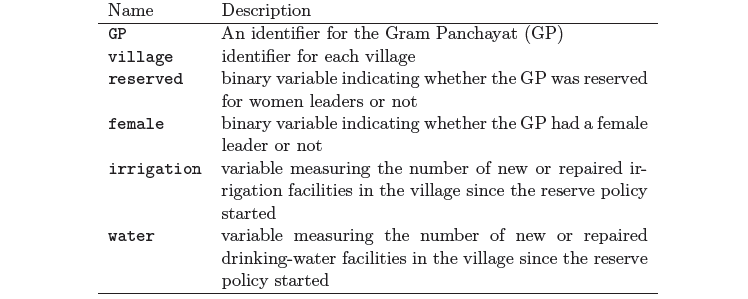
\includegraphics[width=1.1\textwidth]{women_desc.png}
\end{figure}		

\newpage
\begin{enumerate}
	\item [(a)] State a null and alternative (two-tailed) hypothesis. \\
	
\section*{Answers 2 (a)}	
	
	The null hypothesis is that there is no association between the reservation policy in place in each GP for female leaders and the number of new or repaired drinking water facilities in the village. In that case the slope will = 0. \\
	
	The alternative hypothesis states there is a correlation between the reservation policy in place for women leaders in a district (either positive or negative) and the water policies in place. In that case the slope will be greater or less than 0. \\
	
	
	
	\item [(b)] Run a bivariate regression to test this hypothesis in \texttt{R} (include your code!). \\
	
	\section*{Answers 2 (b)}
	
	Looking at the data, there is a high correlation (0.8976907) between GPs that are reserved for women, and the number of females in GPs. 
	
	\begin{verbatim}
		cor(data_India$reserved ==1,data_India$female ==1)
	\end{verbatim}
	
That being the case, this analysis will  run a regression analysis comparing the GPs with female representation and the number of new or repaired water facilities.  
	
	\begin{verbatim}

data_female <- (data_India$female == 1)
data_male <- (data_India$female == 0)

model_water <- summary(lm(data_India$water~data_female))
print(model_water)


Call:
lm(formula = data_India$water ~ data_female)

Residuals:
Min     1Q Median     3Q    Max 
-22.68 -14.78  -7.81   2.29 317.32 

Coefficients:
Estimate Std. Error t value Pr(>|t|)    
(Intercept)       14.813      2.382   6.220 1.56e-09 ***
data_femaleTRUE    7.864      3.838   2.049   0.0413 *  
---
Signif. codes:  
0 ‘***’ 0.001 ‘**’ 0.01 ‘*’ 0.05 ‘.’ 0.1 ‘ ’ 1

Residual standard error: 33.51 on 320 degrees of freedom
Multiple R-squared:  0.01295,	Adjusted R-squared:  0.009867 
F-statistic: 4.199 on 1 and 320 DF,  p-value: 0.04126

	\end{verbatim}
	
We can also plot the association 

	\begin{verbatim}
plot(data_India$water ~ data_female, col = "blue")
abline(coef(lm(data_India$water~data_female)), col = "green")
abline(coef(lm(data_India$water~data_male)), col = "purple")
	\end{verbatim}
	
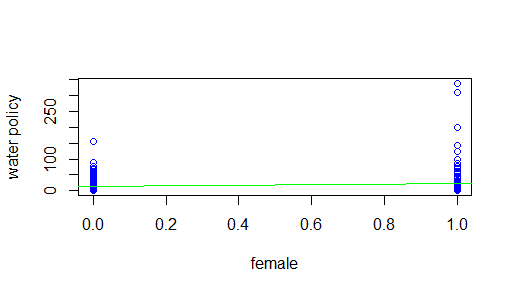
\includegraphics{Rplot_just_green}

	\item [(c)] Interpret the coefficient estimate for reservation policy. \\
	
	\textbf{Answer:} The slope is equal to 7.864, indicating a correlation between female leaders and water policy. 
	
	The P-Value is less than 0.05, so the test can be considered significant, and we have evidence to reject the null hypothesis in this instance.
	
\end{enumerate}

\end{document}
